\documentclass[12pt]{article}
\usepackage{latexblog}

% ============================================================
% Blog Metadata
% ============================================================
\blogtitle{Mac上的C++/CMake开发环境抉择}
\blogdate{2020-04-08}
\blogtags{CMake, 开发环境, 闲话编程, Eclipse, C++}
\bloglang{zh}
\blogsummary{}

\begin{document}
\makeblogtitle

之前写过一篇文章\href{../visual_studio_code_cpp_ide}{Visual Studio Code for C++ development on MacOS}, 因为在Mac上一直没有找到免费且又比较好用的C++开发工具。但相比起Visual Studio而言，Visual Studio Code还是太简陋了。而今时不同往日了，现在比较倾向于使用CMake来构建项目，所以希望能支持CMake，所以又把各种开发工具尝试了一下。

\section{Eclipse CDT}\label{eclipse-cdt}

最近Eclipse-CDT又更新了一下，再次体验了一下，而且根据之前的经验，eclipse是直接支持CMake了的，所以是我的首选目标。

\subsection{导入CMake工程}\label{ux5bfcux5165cmakeux5de5ux7a0b}

Eclipse CDT默认是支持CMake的，所以不用使用cmake生成eclipse的工程，直接就可以用。新建项目的时候是可以直接选用CMake项目的，那么，怎么导入一个现有的CMake工程呢？

实际上，并不能使用''Import''来导入，而是要用''File -\textgreater{} New -\textgreater{} C/C++ Project -\textgreater{} Empty or Existing CMake Project''，然后就可以选择现有项目，导入到Eclipse中去了。是不是很坑？

\begin{figure}
\centering
\pandocbounded{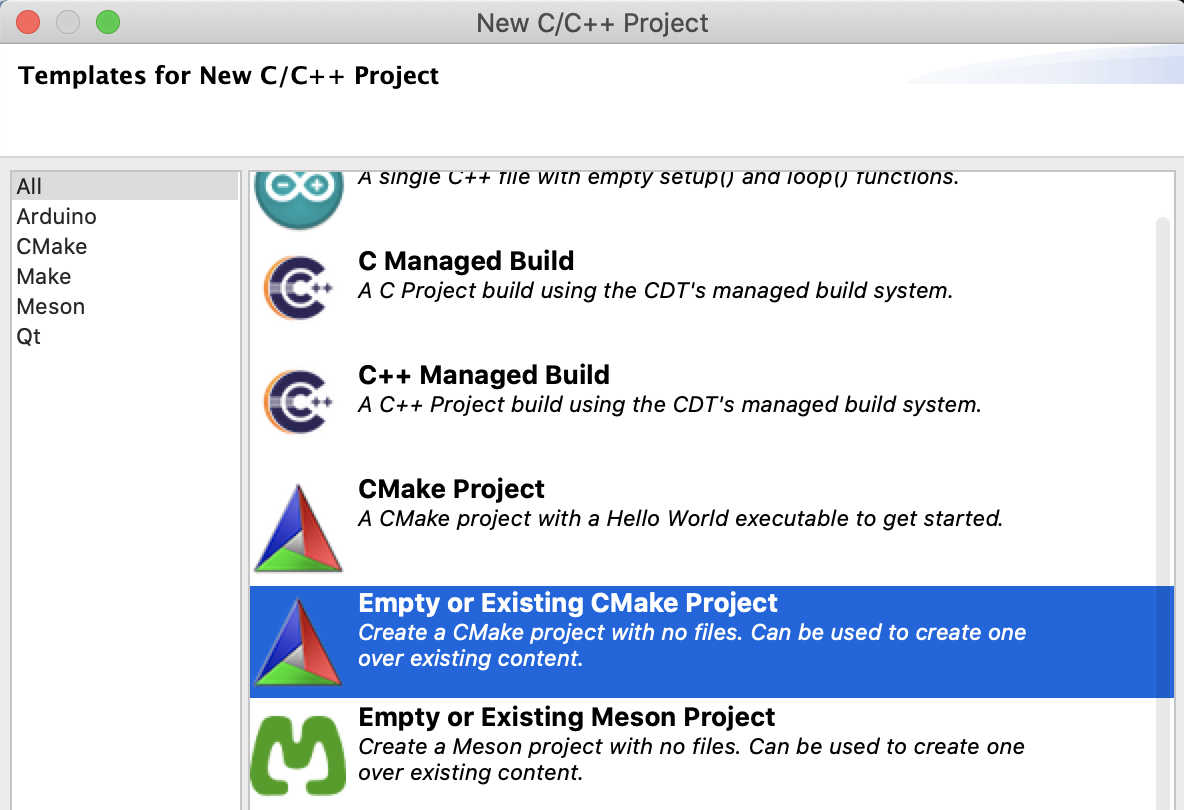
\includegraphics[keepaspectratio,alt={Import project}]{images/CDT_import_cmake_project.png}}
\caption{Import project}
\end{figure}

\subsection{运行Google Test测试}\label{ux8fd0ux884cgoogle-testux6d4bux8bd5}

可以直接在Eclipse中运行Google Test，因为本身编译测试出来是一个应用，其实可以直接运行，但是eclipse集成的Unit Test可以让结果更好看一点：

\begin{figure}
\centering
\pandocbounded{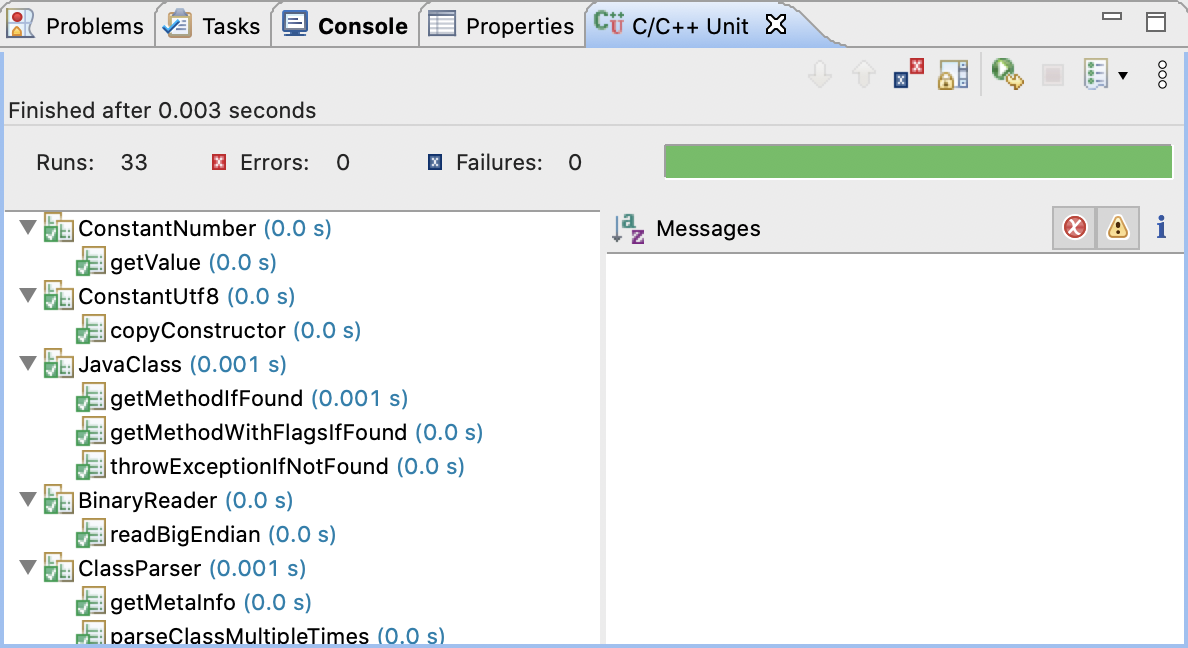
\includegraphics[keepaspectratio,alt={Run tests}]{images/CDT_run_tests.png}}
\caption{Run tests}
\end{figure}

要运行这样的测试必须在Run Configuration中新建一个Unit Test的目标，并选择编译出来的test程序。

\subsection{Mac下字体设置}\label{macux4e0bux5b57ux4f53ux8bbeux7f6e}

Eclipse在Mac下有一个问题就是默认的UI字体实在太小了，看着眼睛疼。

\begin{figure}
\centering
\pandocbounded{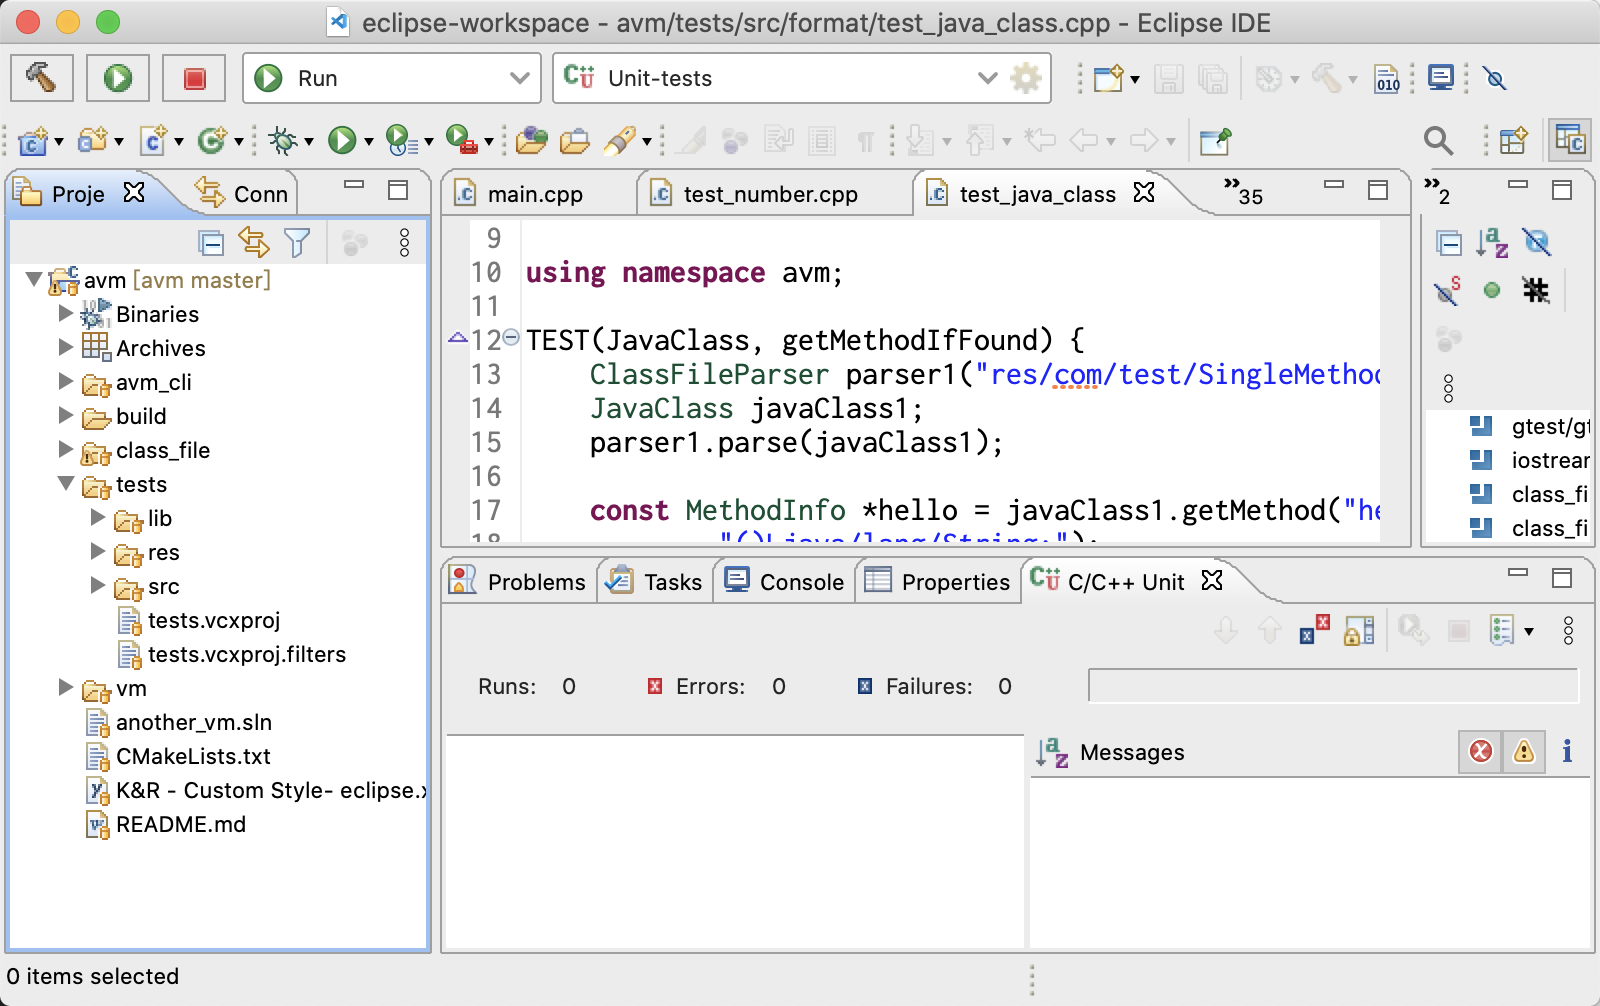
\includegraphics[keepaspectratio,alt={默认字体}]{images/CDT_smallfont.png}}
\caption{默认字体}
\end{figure}

有一个解决办法就是安装一个\href{https://www.bresink.com/osx/TinkerTool.html}{TinkerTool}，然后设置``Help tags''字体的大小。参见这个\href{https://bugs.eclipse.org/bugs/show_bug.cgi?id=56558}{Bug}。

\begin{figure}
\centering
\pandocbounded{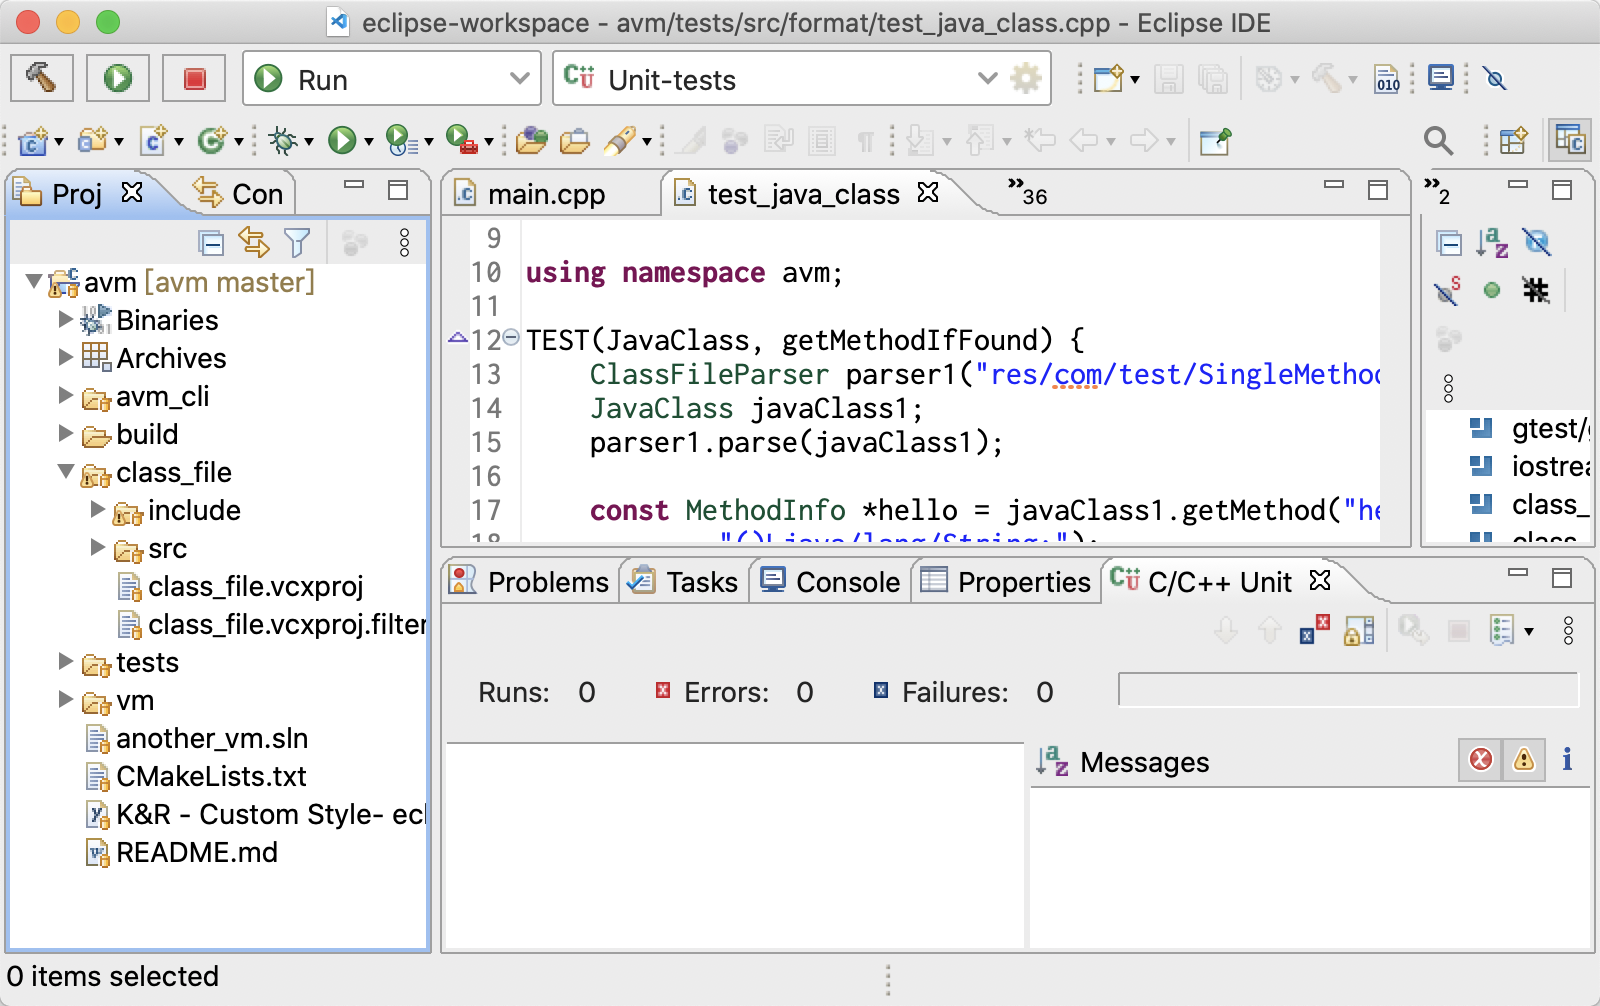
\includegraphics[keepaspectratio,alt={更改后的字体}]{images/CDT_14px.png}}
\caption{更改后的字体}
\end{figure}

\subsection{缺点}\label{ux7f3aux70b9}

也许Eclipse最大的问题就在于调试了，动不动就卡死在96\%上，或者好不容易进去了，却告诉你没有调试信息，要不要看汇编？尝试了很久也没有找到解决办法，除此之外，别的都能接受。但是这个问题很致命啊\ldots{} 另外一个问题就是，（即使gdb支持的也不好），eclipse是不直接支持lldb的。

\section{Visual Studio Code}\label{visual-studio-code}

看来还是把希望寄托在Visual Studio Code上了。

\subsection{安装插件}\label{ux5b89ux88c5ux63d2ux4ef6}

有以下的几个插件需要安装：

\begin{itemize}
\tightlist
\item
  ms-vscode.cpptools: C/C++插件
\item
  ms-vscode.cmake-tools: CMake tools
\item
  webfreak.debug: Native debug插件
\end{itemize}

安装完成之后，就可以打开CMake工程了。使用Command+Shift+P打开命令窗口，可以看到有很多CMake相关的选项：

\begin{itemize}
\tightlist
\item
  CMake:Configure 配置支持CMake工程
\item
  CMake:Clean 清理build
\item
  \ldots{}
\end{itemize}

也可以通过系统下面的状态栏来设置，设置好之后，一般长这个样子：

\begin{figure}
\centering
\pandocbounded{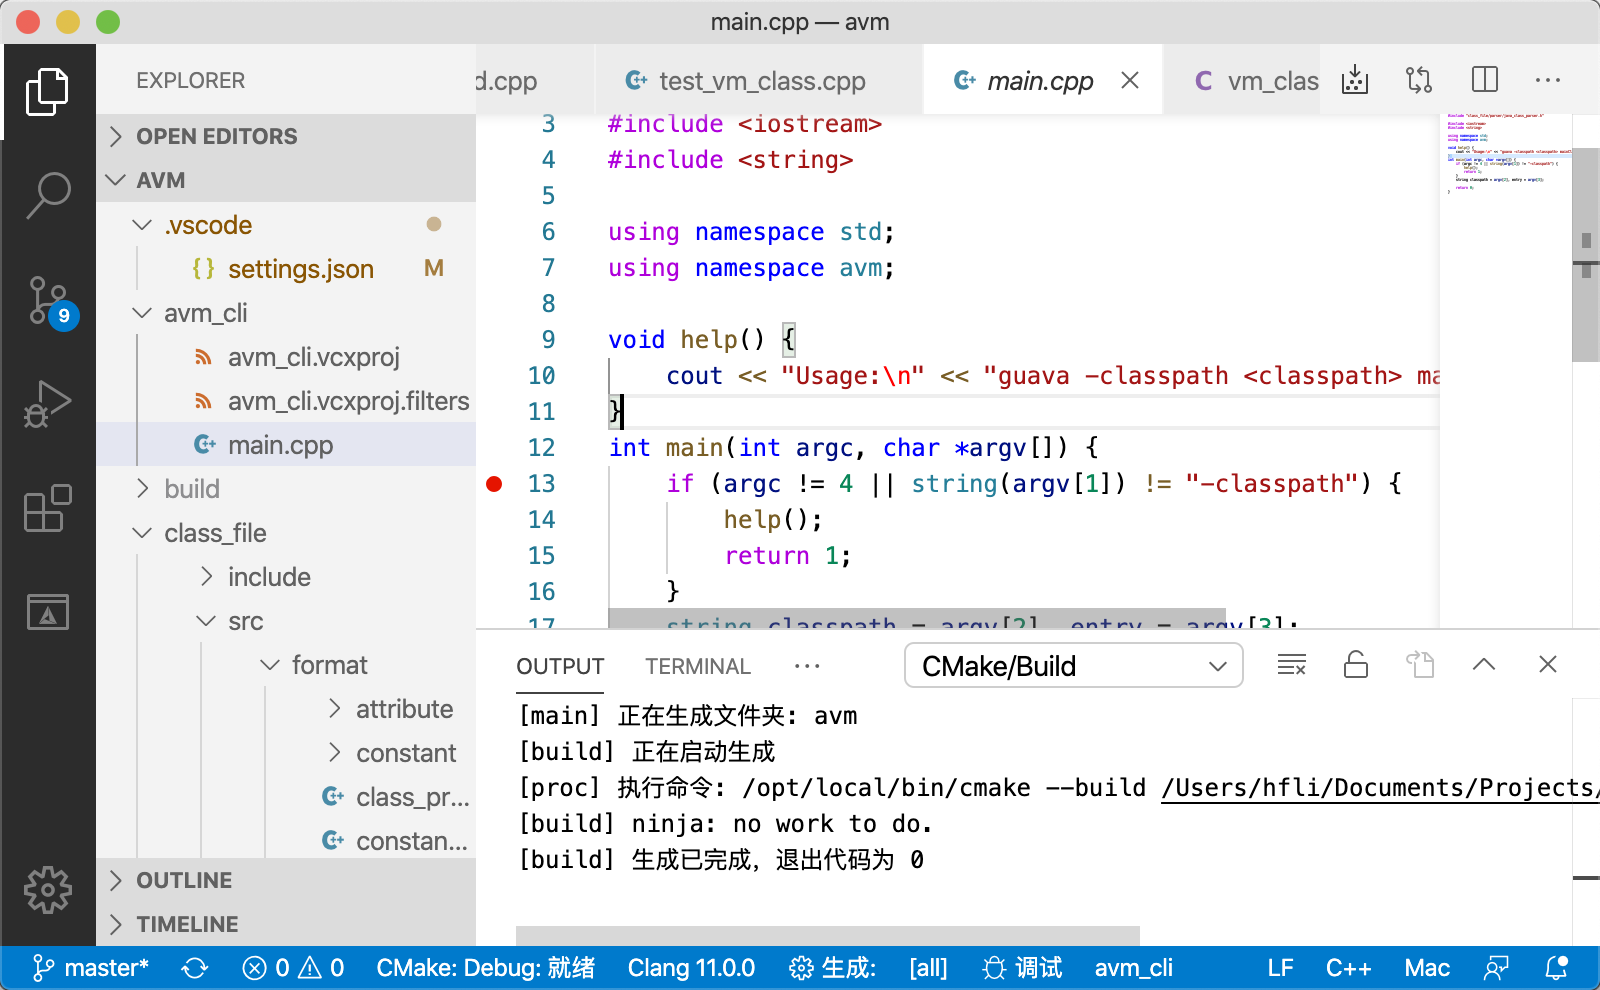
\includegraphics[keepaspectratio,alt={Visual Studio Code}]{images/Vscode-cmaketools.png}}
\caption{Visual Studio Code}
\end{figure}

可以看到下面的状态栏已经集成了CMake的target。

\subsection{调试}\label{ux8c03ux8bd5}

\subsubsection{使用lldb-mi从状态栏启动调试}\label{ux4f7fux7528lldb-miux4eceux72b6ux6001ux680fux542fux52a8ux8c03ux8bd5}

调试有两种方式：一种是通过状态栏下面的''调试``图标启动的，不需要launch.json，但是默认情况下是不能工作的，需要做如下设置：

新建\texttt{.vscode/settings.json}，将cpptools下面lldb-mi的路径配置进去，比如我的：

\begin{Shaded}
\begin{Highlighting}[]
\FunctionTok{\{}
    \DataTypeTok{"cmake.debugConfig"}\FunctionTok{:} \FunctionTok{\{}
        \DataTypeTok{"miDebuggerPath"}\FunctionTok{:} \StringTok{"/Users/hfli/.vscode/extensions/ms{-}vscode.cpptools{-}0.27.0/debugAdapters/lldb{-}mi/bin/lldb{-}mi"}
    \FunctionTok{\}}
\FunctionTok{\}}
\end{Highlighting}
\end{Shaded}

\begin{figure}
\centering
\pandocbounded{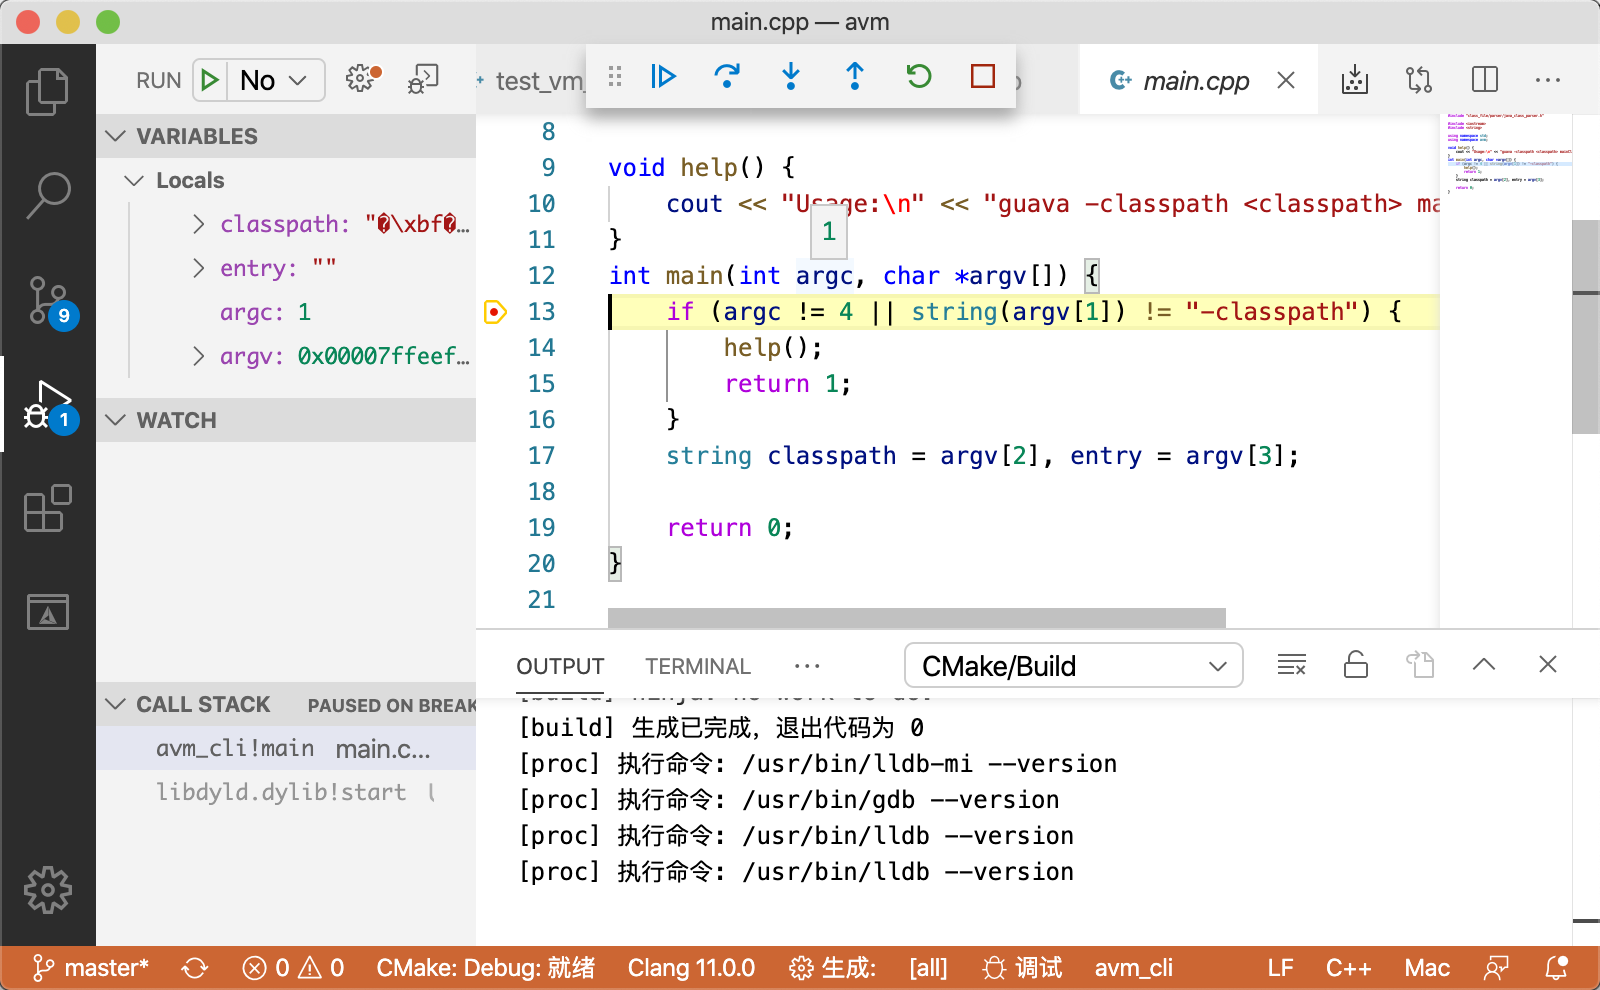
\includegraphics[keepaspectratio,alt={lldb-mi}]{images/Vscode-debug-lldb-mi.png}}
\caption{lldb-mi}
\end{figure}

但是这个玩意感觉支持很有限，我调试Googletest测试的的时候就直接挂掉了。

\subsubsection{创建launch.json调试}\label{ux521bux5efalaunch.jsonux8c03ux8bd5}

另外一个方式是创建launch.json，这样可以从左边的调试菜单那里开始：

\begin{Shaded}
\begin{Highlighting}[]
\FunctionTok{\{}
    \DataTypeTok{"version"}\FunctionTok{:} \StringTok{"0.2.0"}\FunctionTok{,}
    \DataTypeTok{"configurations"}\FunctionTok{:} \OtherTok{[}
        \FunctionTok{\{}
            \DataTypeTok{"name"}\FunctionTok{:} \StringTok{"(gdb) Launch"}\FunctionTok{,}
            \DataTypeTok{"type"}\FunctionTok{:} \StringTok{"cppdbg"}\FunctionTok{,}
            \DataTypeTok{"request"}\FunctionTok{:} \StringTok{"launch"}\FunctionTok{,}
            \ErrorTok{//} \ErrorTok{Resolved} \ErrorTok{by} \ErrorTok{CMake} \ErrorTok{Tools}\FunctionTok{:}
            \StringTok{"program"}\ErrorTok{:} \StringTok{"$\{command:cmake.launchTargetPath\}"}\FunctionTok{,}
            \DataTypeTok{"args"}\FunctionTok{:} \OtherTok{[]}\FunctionTok{,}
            \DataTypeTok{"stopAtEntry"}\FunctionTok{:} \KeywordTok{false}\FunctionTok{,}
            \DataTypeTok{"cwd"}\FunctionTok{:} \StringTok{"$\{workspaceFolder\}/build"}\FunctionTok{,}
            \DataTypeTok{"environment"}\FunctionTok{:} \OtherTok{[]}\FunctionTok{,}
            \DataTypeTok{"externalConsole"}\FunctionTok{:} \KeywordTok{true}\FunctionTok{,}
            \DataTypeTok{"MIMode"}\FunctionTok{:} \StringTok{"gdb"}\FunctionTok{,}
            \DataTypeTok{"MIDebuggerPath"}\FunctionTok{:} \StringTok{"/Users/hfli/.vscode/extensions/ms{-}vscode.cpptools{-}0.27.0/debugAdapters/lldb{-}mi/bin/lldb{-}mi"}\FunctionTok{,}
            \DataTypeTok{"setupCommands"}\FunctionTok{:} \OtherTok{[}
                \FunctionTok{\{}
                    \DataTypeTok{"description"}\FunctionTok{:} \StringTok{"Enable pretty{-}printing for gdb"}\FunctionTok{,}
                    \DataTypeTok{"text"}\FunctionTok{:} \StringTok{"{-}enable{-}pretty{-}printing"}\FunctionTok{,}
                    \DataTypeTok{"ignoreFailures"}\FunctionTok{:} \KeywordTok{true}
                \FunctionTok{\}}
            \OtherTok{]}
        \FunctionTok{\}}
    \OtherTok{]}
\FunctionTok{\}}
\end{Highlighting}
\end{Shaded}

但上面照样使用的是lldb-mi，有着跟上面的方法同样的问题。换成gdb后就更是奇怪的到处乱跳了。

\subsubsection{使用CodeLLDB插件}\label{ux4f7fux7528codelldbux63d2ux4ef6}

另一个选项就是使用CodeLLDB插件，安装完成之后配置\texttt{launch.json}：

\begin{Shaded}
\begin{Highlighting}[]
\FunctionTok{\{}
    \DataTypeTok{"version"}\FunctionTok{:} \StringTok{"0.2.0"}\FunctionTok{,}
    \DataTypeTok{"configurations"}\FunctionTok{:} \OtherTok{[}
        \FunctionTok{\{}
            \DataTypeTok{"name"}\FunctionTok{:} \StringTok{"Launch debug"}\FunctionTok{,}
            \DataTypeTok{"type"}\FunctionTok{:} \StringTok{"lldb"}\FunctionTok{,}
            \DataTypeTok{"request"}\FunctionTok{:} \StringTok{"launch"}\FunctionTok{,}
            \DataTypeTok{"program"}\FunctionTok{:} \StringTok{"$\{command:cmake.launchTargetPath\}"}\FunctionTok{,}
            \DataTypeTok{"args"}\FunctionTok{:} \OtherTok{[]}\FunctionTok{,}
            \DataTypeTok{"stopAtEntry"}\FunctionTok{:} \KeywordTok{false}\FunctionTok{,}
            \DataTypeTok{"cwd"}\FunctionTok{:} \StringTok{"$\{workspaceFolder\}/build"}\FunctionTok{,}
            \DataTypeTok{"environment"}\FunctionTok{:} \OtherTok{[]}
        \FunctionTok{\}}
    \OtherTok{]}
\FunctionTok{\}}
\end{Highlighting}
\end{Shaded}

这样终于不会在我调试googletest的时候死掉了，

\begin{figure}
\centering
\pandocbounded{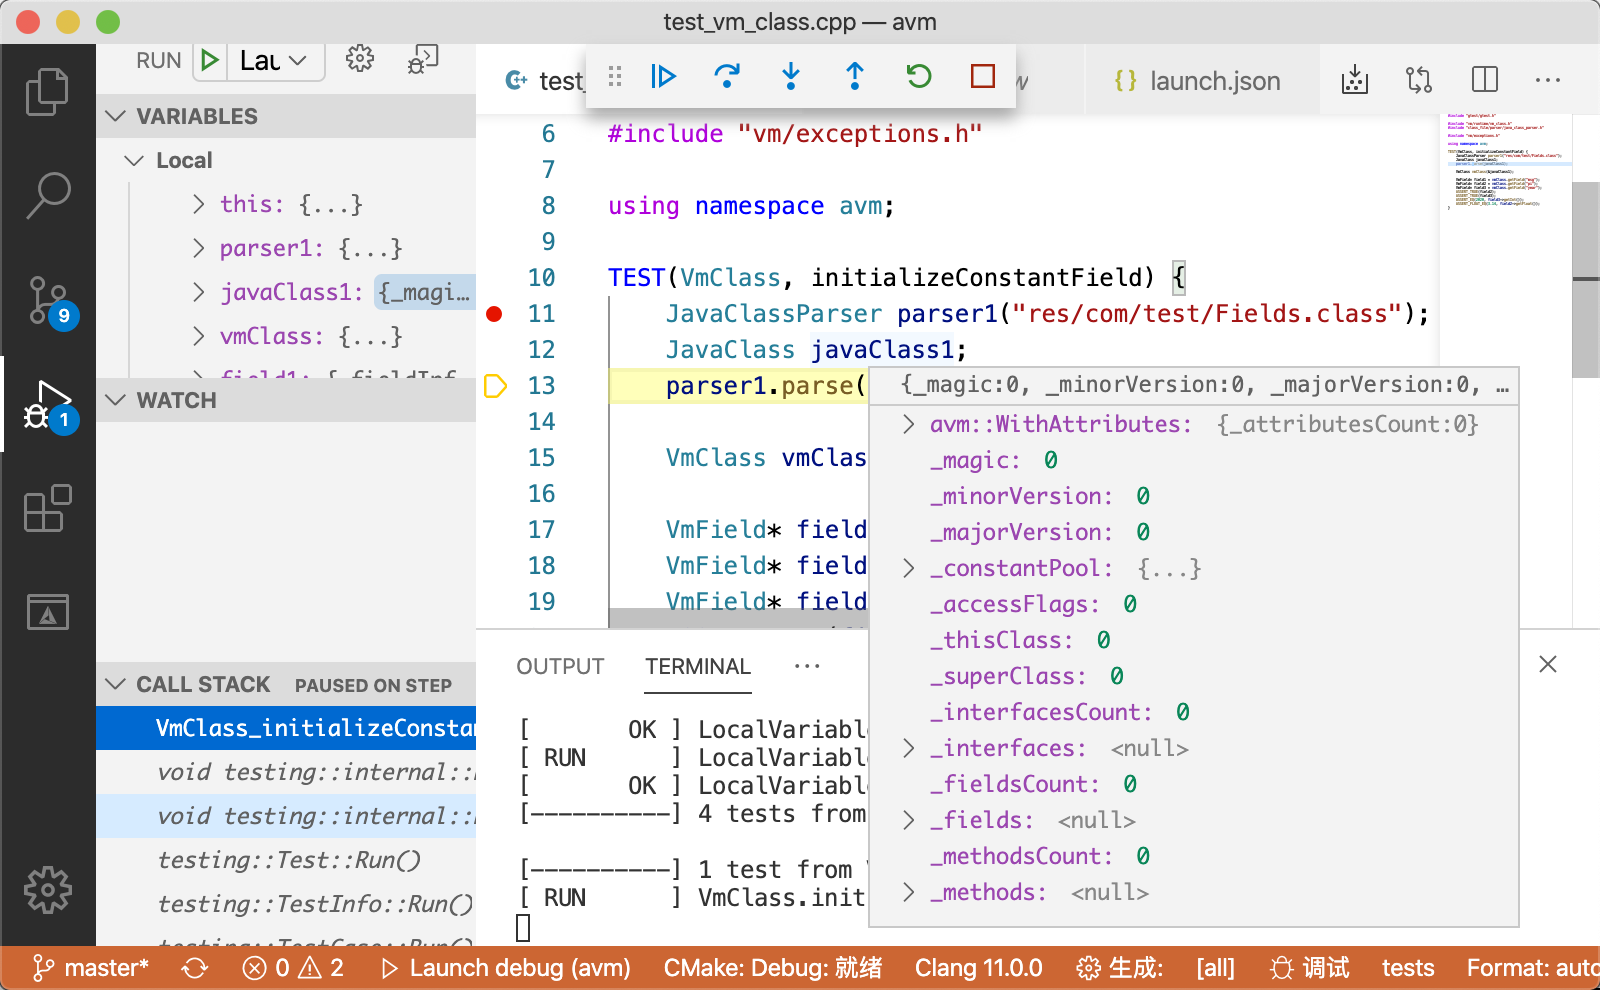
\includegraphics[keepaspectratio,alt={CodeLLDB}]{images/Vscode-debug-codelldb.png}}
\caption{CodeLLDB}
\end{figure}

\section{Qt Creator}\label{qt-creator}

\section{KDevelop}\label{kdevelop}

\begin{itemize}
\tightlist
\item
  \href{https://github.com/microsoft/vscode-cmake-tools/issues/965}{Can't debug in Visual Studio Code \#965}
\item
  \href{https://vector-of-bool.github.io/docs/vscode-cmake-tools/debugging.html\#debugging}{Target Debugging and Launching}
\end{itemize}


\end{document}
